\documentclass[10pt]{article}
\usepackage[polish]{babel}
\usepackage[utf8]{inputenc}
\usepackage[T1]{fontenc}
\usepackage{amsmath}
\usepackage{amsfonts}
\usepackage{amssymb}
\usepackage[version=4]{mhchem}
\usepackage{stmaryrd}
\usepackage{graphicx}
\usepackage[export]{adjustbox}
\graphicspath{ {./images/} }
\usepackage{bbold}

\title{LIGA MATEMATYCZNA \\
 FINAE \\
 26 marca 2010 \\
 SZKOŁA PONADGIMNAZJALNA }

\author{}
\date{}


\begin{document}
\maketitle
\section*{ZADANIE 1.}
Wykaż, że jeżeli w trapez można wpisać okrąg, to okręgi, których średnicami są ramiona tego trapezu, są styczne.

\section*{ZADANIE 2.}
Udowodnij, że jeśli \(p\) i \(q\) są liczbami pierwszymi takimi, że \(p \geqslant 5\) oraz \(q-p=2\), to liczba \(p+q\) jest podzielna przez 12.

\section*{ZADANIE 3.}
Pole trójkąta \(E F G\) jest równe 1. Oblicz pole trójkąta \(A B C\), wiedząc, że

\[
|A E|=|E G|,|E F|=|F B|,|F G|=|G C| .
\]

\begin{center}
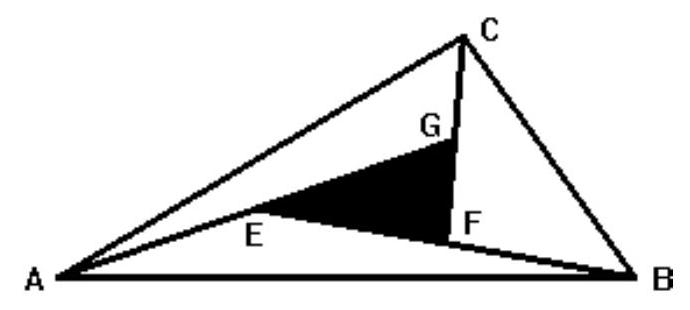
\includegraphics[max width=\textwidth]{2024_11_21_4d8e2eb8935e7b6d3c11g-1}
\end{center}

\section*{ZADANIE 4.}
Znajdź wszystkie funkcje \(f: \mathbb{R} \rightarrow \mathbb{R}\) spełniające warunek

\[
f(x) f(y)-f(x y)=x+y \text { dla wszystkich liczb rzeczywistych } x, y
\]

\section*{ZADANIE 5.}
Oblicz wartość wyrażenia \(q^{4}-6 q^{3}+9 q^{2}-7\) wiedząc, że \(q^{2}-3 q+1=0\).

\section*{ZADANIE 6.}
Przedstaw liczbę 1 jako sumę kwadratów: (a) dwóch; (b) trzech; (c) czterech, parami różnych dodatnich liczb wymiernych.

\section*{ZADANIE 7.}
Na okręgu zaznaczono sześć punktów. Każdy z odcinków łączących te punkty pomalowano na czerwono lub niebiesko. Wykaż, że otrzymano przynajmniej jeden jednokolorowy trójkąt.


\end{document}